% Author: Alvin Thai
%         Nicholas Pelham
% Source: CS122A Project

\documentclass{standalone}

\usepackage{pgf}
\usepackage{tikz}
\usetikzlibrary{arrows, automata, positioning}
\usepackage[latin1]{inputenc}

\begin{document}

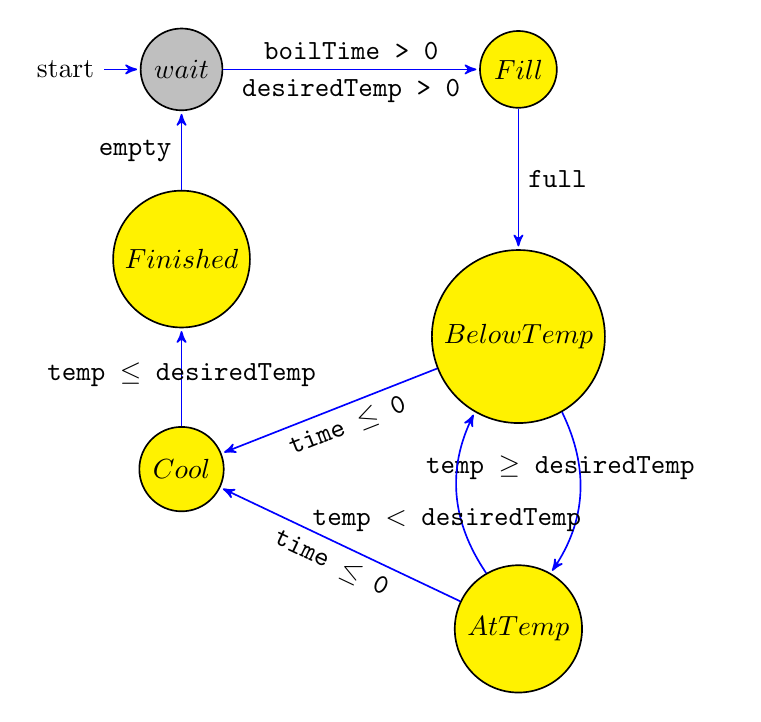
\begin{tikzpicture}[->, >=stealth', shorten >=1pt, auto, node distance=2.8cm,
                    semithick, draw=blue]
  \tikzstyle{every state}=[fill=yellow, draw=black, text=black]

  \node[initial,state] (A) [fill=lightgray, draw=black, text=black] {$wait$};
  \node[state]         (B) [right =3.25cm of A]                      {$Fill$};
  \node[state]         (C) [below =1.785cm of B]                    {$BelowTemp$};
  \node[state]         (D) [below =1.785cm of C]                    {$AtTemp$};
  \node[state]         (E) [below =4cm of A]                        {$Cool$};
  \node[state]         (F) [below =1cm of A]                        {$Finished$};

  \path 
        (A) edge [draw=blue]                   node [sloped, above]{\texttt{boilTime > 0}} 
                                               node [sloped, below]{\texttt{desiredTemp > 0}}(B)
        (B) edge [draw=blue]                   node {\texttt{full}} (C)
        (C) edge [draw=blue, bend left]        node [below, pos=0.2]{\texttt{temp $\geq$ desiredTemp~~~}} (D)
        (D) edge [draw=blue, bend left]        node [above, pos=0.2]{\texttt{temp $<$ desiredTemp~~~~}} (C)
        (C) edge [draw=blue]                   node [sloped, below, pos=0.45]{\texttt{time $\leq$ 0}} (E)
        (D) edge [draw=blue]                   node [sloped, below]{\texttt{time $\leq$ 0}} (E)
        (E) edge [draw=blue]                   node [above, pos=0.3]{\texttt{temp $\leq$ desiredTemp}} (F)
        (F) edge [draw=blue]                   node {\texttt{empty}} (A);
\end{tikzpicture}

\end{document}